%- - - - - - - - - - - - - - - - - - - - - - - - - - - - - - - - - SLIDE -
\begin{frame}
\frametitle{Complete Search}
\begin{block}{}
\begin{itemize}
	\bitem Estratégia baseada no princípio KISS (``Keep It Simple, Stupid'')
	\begin{itemize}
		\bitem Buscar os resultados evitando qualquer complexidade desnecessária.
	\end{itemize}
	\bitem O objetivo numa competição de programação é escrever um programa que resolva o problema dentro do tempo limite.
	\begin{itemize}
		\bitem Não importa se existe ou não uma solução mais eficiente.
	\end{itemize}
	\bitem A busca exaustiva faz uso do método trivial, de força bruta, todas as possíveis soluções são analisadas para encontrar a resposta.
	\bitem Essa técnica sempre deve ser a primeira a ser considerada.
	\begin{itemize}
		\bitem Caso funcione dentro do limite de tempo / memória, use-a! 
		\begin{itemize}
			\bitem Geralmente é fácil de codificar e debugar.
%			\bitem Mais tempo para trabalhar nos problemas difíceis. 
		\end{itemize}
	\end{itemize}
	\bitem Apenas alguns milhões de possíveis respostas para um problema? Itere em todas elas e encontre aquela que funciona.
\end{itemize}
\end{block}
\pause

\begin{block}{\tiny Cuidado!!}
Nem sempre é óbvio que a busca exaustiva pode ser usada.
\end{block}
\end{frame}

%- - - - - - - - - - - - - - - - - - - - - - - - - - - - - - - - - SLIDE -
\begin{frame}
\frametitle{Complete Search}

\begin{block}{}
\begin{itemize}
	\bitem Uma das técnicas de resolução de problemas mais importantes;
	\begin{itemize}
		\bitem Pode ser aplicada a uma grande gama de problemas quando as instâncias são pequenas os suficiente
		\bitem Ponto de partida para o desenvolvimento de outros algoritmos.
	\end{itemize}
	\bitem Competidor precisa saber:
	\begin{itemize}
		\bitem Gerar/testar: subconjuntos, permutações, ...
		\bitem Técnicas para reduzir o espaço de busca
		\bitem Estimar a complexidade no pior caso
	\end{itemize}
	\bitem Ajustes no código podem influenciar bastante no tempo de execução;
	\begin{itemize}
		\bitem Vale a pena implementar a mesma solução de formas diferentes.
	\end{itemize}
\end{itemize}	
\end{block}

\begin{block}{\tiny \#protip}
Quando não conseguir pensar em um jeito melhor de resolver o problema arrisque a solução por força bruta.
Caso exista um caso onde ela não é rápida o suficiente, mantenha a solução por perto e use-a para testar outras soluções nos casos menores.
\end{block}
\end{frame}

%- - - - - - - - - - - - - - - - - - - - - - - - - - - - - - - - - SLIDE -
\begin{frame}
\frametitle{Complete Search}
\begin{block}{Filtrar vs. Gerar }
Duas possíveis abordagens podem ser escolhidas quando fazendo uma busca exaustiva:
\begin{itemize}
	\bitem Filtragem -- Todas as possíveis soluções são geradas e depois examinadas para eliminar as inválidas.
	\bitem Geração -- Soluções construídas progressivamente, assim que uma inconsistência é detectada a solução é descartada.
\end{itemize}
\end{block}
\pause
\begin{block}{}
\begin{itemize}
	\bitem Candidato parcial (estado) -- parte de uma possível solução;
	\begin{itemize}
		\bitem Pode ser completado (através de um passo de extensão) de diferentes maneiras para gerar uma solução.
	\end{itemize}	
	\bitem Candidatos são os nós de uma árvore. Cada candidato parcial é pai dos candidatos que podem ser obtidos a partir dele em um passo de extensão.
\end{itemize}
\end{block}
\end{frame}

%- - - - - - - - - - - - - - - - - - - - - - - - - - - - - - - - - SLIDE -
\begin{frame}
\frametitle{Complete Search}
\begin{center}
\begin{figure}
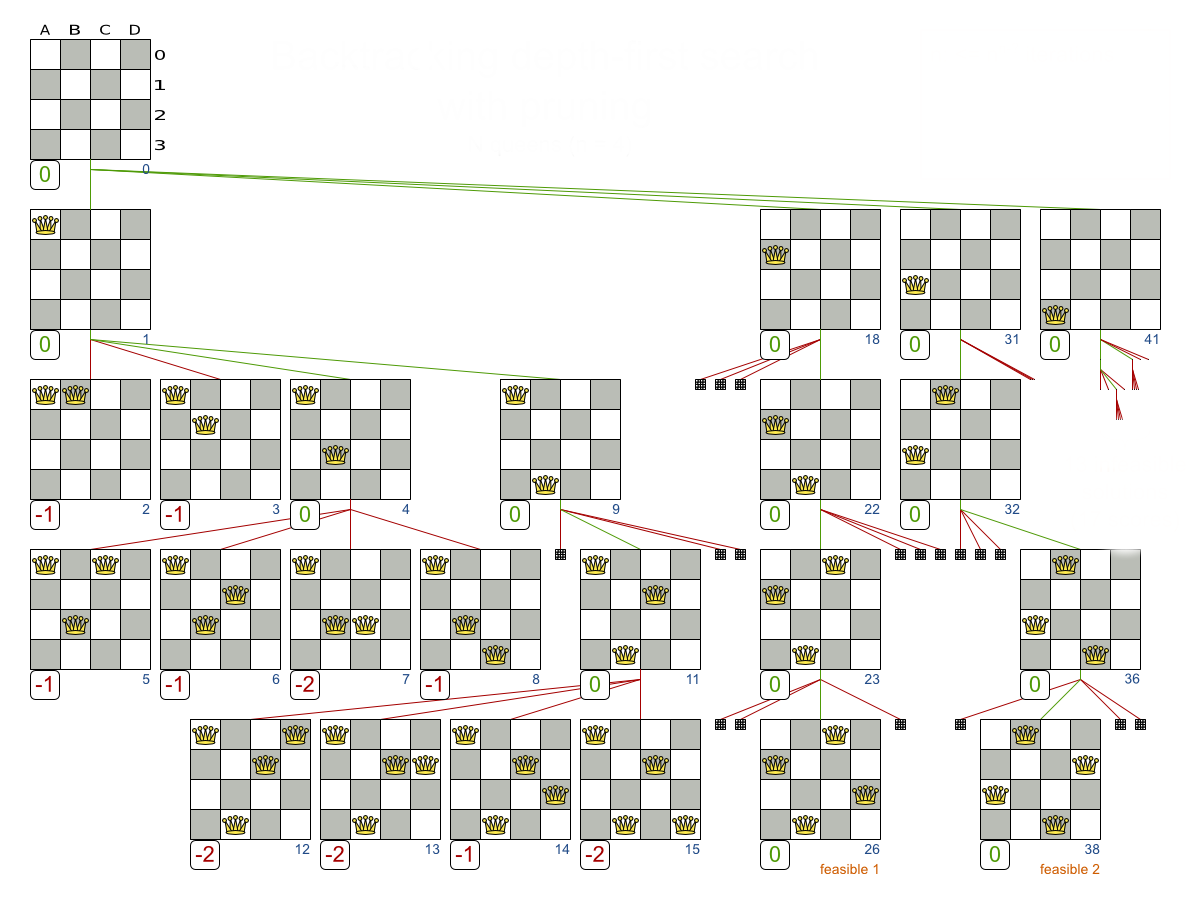
\includegraphics[width=.9\textwidth]{figuras/backtrackingDepthFirstSearchNQueens.png}
\end{figure}
\end{center}
\end{frame}

%- - - - - - - - - - - - - - - - - - - - - - - - - - - - - - - - - SLIDE -
\begin{frame}
\frametitle{Complete Search}
\begin{block}{Problema: $n$ Queens}
\scriptsize
Colocar $n$ rainhas em um tabuleiro de xadrez $n\ x\ n$ de modo que uma rainha não ataque outra.
\end{block}
\pause
\begin{block}{Abordagens..}
\begin{itemize}[<+->]
	\bitem 1. Gerar $n$ pares $(x,y)$ e verificar se formam uma solução válida.
	\begin{itemize}
		\item[] $n^{2n}$ -- \textbf{\textcolor{red}{BAD!}}
	\end{itemize}
	\bitem \texttt{$Obs_1$.: Cada coluna deve ter exatamente uma rainha..}
	\bitem 2. Gerar as $n^n$ possíveis soluções e verificar se são válidas.
	\begin{itemize}
		\item[] \textbf{Melhorou, só que não!}
	\end{itemize}
	\bitem \texttt{$Obs_2$.: Cada linha também tem exatamente uma rainha..}
	\bitem 3. Gerar as $n!$ possíveis soluções e verificar se são válidas.
	\begin{itemize}
		\item[] \textbf{Hmm, parece ``bom''.. será que dá pra melhorar?}
	\end{itemize}
\end{itemize}
\end{block}
\end{frame}

%- - - - - - - - - - - - - - - - - - - - - - - - - - - - - - - - - SLIDE -
\begin{frame}
\frametitle{Complete Search}
\begin{block}{Problema: $n$ Queens}
\scriptsize
Colocar $n$ rainhas em um tabuleiro de xadrez $n\ x\ n$ de modo que uma rainha não ataque outra.
\end{block}

\begin{block}{Busca em profundidade, Backtracking}
\begin{itemize}[<+->]
	\bitem Podemos tentar adicionar as rainhas uma por uma, recursivamente, no tabuleiro.
	\bitem Explorando o fato de que é necessário colocar uma rainha por coluna, em cada passo da recursão basta escolher em qual linha na coluna atual colocar a rainha.
	\bitem Não faz sentido colocar uma rainha em uma posição que entra na zona de ataque de alguma das rainhas anteriormente colocadas.
	\bitem Continuamos tentando gerar as $n!$ permutações, mas agora só geramos aquelas que são válidas. \color{ccomments}{(filtrar vs. gerar)}
\end{itemize}
\end{block}
\end{frame}

%- - - - - - - - - - - - - - - - - - - - - - - - - - - - - - - - - SLIDE -
\begin{frame}
\frametitle{Complete Search}
\begin{block}{Problema: $n$ Queens}
\scriptsize
Colocar $n$ rainhas em um tabuleiro de xadrez $n\ x\ n$ de modo que uma rainha não ataque outra.
\end{block}

\begin{block}{Busca em profundidade, Backtracking}
\includefile{c++}{codes}{pseudonqueen.cpp}
\end{block}
\end{frame}

%- - - - - - - - - - - - - - - - - - - - - - - - - - - - - - - - - SLIDE -
\begin{frame}
\frametitle{Complete Search}

\begin{block}{Busca em profundidade, Backtracking}

\begin{itemize}
	\bitem Essa abordagem é um exemplo de uma busca em profundidade (DFS - \emph{Depth First Search})
	\begin{itemize}
		\bitem O algoritmo tenta iterar do topo ao fundo da árvore o mais rápido possível.
		\bitem Um vez que $k$ rainhas são colocadas no tabuleiro, apenas tabuleiros com mais rainhas são examinados.
	\end{itemize}
	\bitem O algoritmo busca na árvore de cima para baixo, analisando os candidatos parciais.
	\bitem Quando uma solução é encontrada ou uma inconsistência detectada, o mecanismo de \emph{backtracking} entra em ação
	\begin{itemize}
		\bitem O caminho que levou até aquela solução é percorrido ao contrário até que uma nova extensão possa ser gerada.
	\end{itemize}
\end{itemize}
\end{block}
\end{frame}

%- - - - - - - - - - - - - - - - - - - - - - - - - - - - - - - - - SLIDE -
\begin{frame}
\frametitle{Complete Search}
	\begin{center}
		\begin{figure}
			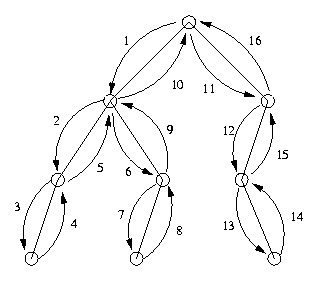
\includegraphics[width=.52\textwidth]{figuras/dfs.png}
			\caption{USACO}
		\end{figure}
	\end{center}
\end{frame}

%- - - - - - - - - - - - - - - - - - - - - - - - - - - - - - - - - SLIDE -
\begin{frame}
\frametitle{Complete Search}

\begin{block}{Busca em profundidade, Backtracking - Complexidade}

\begin{itemize}
	\bitem Seja $d$ o número de decisões que devem ser feitas 
	\begin{itemize}
		\item[] \scriptsize{No caso das $n$-rainhas $d=n$, o nro. de colunas que devemos preencher.}
	\end{itemize}
	\bitem Seja $C$ a quantidade de escolhas para cada decisão
	\begin{itemize}
		\item[] \scriptsize{No caso das $n$-rainhas $C=n$, já que qualquer uma das linhas pode ser escolhida.}
	\end{itemize}
	\bitem No pior caso, a busca leva tempo $O(C^d)$, ou seja, uma quantidade exponencial de tempo.
	\bitem Entretanto, a quantidade de espaço necessária é bem pequena.
	\begin{itemize}
		\bitem Como só é necessário manter informação das decisões a serem feitas, apenas $O(d)$ espaço é necessário.
	\end{itemize}
\end{itemize}
\end{block}
\end{frame}

%- - - - - - - - - - - - - - - - - - - - - - - - - - - - - - - - - SLIDE -
\begin{frame}
\frametitle{Complete Search}
\begin{block}{Problema: Knight Cover}
\scriptsize
Colocar o menor número de cavalos em um tabuleiro de xadrez $n\ x \ n$ de modo que toda célula do tabuleiro está sob ataque.
\tiny{\emph{*Um cavalo não ataca a posição onde ele se encontra.}}
\end{block}
\pause
\begin{block}{Busca em Largura}
\begin{itemize}[<+->]
	\bitem Como queremos o menor número de cavalos, é mais interessante examinar todas as soluções com $k$ cavalos
	antes de partir para aquelas com $k+1$.
	\bitem Essa abordagem é um exemplo de uma busca em largura (BFS - \emph{Breadth First Search})
	\bitem Geralmente a implementação envolve uma fila de estados / candidatos parciais
\end{itemize}
\end{block}
\end{frame}

%- - - - - - - - - - - - - - - - - - - - - - - - - - - - - - - - - SLIDE -
\begin{frame}
\frametitle{Complete Search}
	\begin{center}
		\begin{figure}
			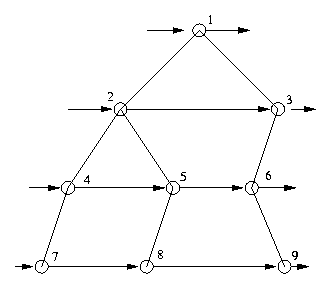
\includegraphics[width=.52\textwidth]{figuras/bfs.png}
			\caption{USACO}
		\end{figure}
	\end{center}
\end{frame}

%- - - - - - - - - - - - - - - - - - - - - - - - - - - - - - - - - SLIDE -
\begin{frame}
\frametitle{Complete Search}
\begin{block}{Busca em Largura}
\includefile{c++}{codes}{pseudobfs.cpp}
\end{block}
\end{frame}

%- - - - - - - - - - - - - - - - - - - - - - - - - - - - - - - - - SLIDE -
\begin{frame}
\frametitle{Complete Search}
\begin{block}{Busca em largura}
\begin{itemize}
	\bitem Chamada de busca em largura porque percorre uma linha inteira (a largura) da árvore de candidatos antes de passar para a próxima linha.
	\bitem Primeiro visita a raiz, então todos os nós no nível 1, depois todos no nível 2, ...
\end{itemize}
\end{block}
\pause
\begin{block}{Busca em largura -- Complexidade}
\begin{itemize}
	\bitem Complexidade de tempo é a mesma da busca em profundidade.
	\bitem Consumo de espaço proporcional ao número de candidatos.
	\begin{itemize}
		\bitem Sejam $c$ o número de escolhas para cada decisão, e $k$ o número de decisões que devem ser feitas.
		\bitem Existem $c^k$ possíveis candidatos que vão estar na fila para o próximo passo.
	\end{itemize}
\end{itemize}
\end{block}
\end{frame}

%- - - - - - - - - - - - - - - - - - - - - - - - - - - - - - - - - SLIDE -
\begin{frame}
\frametitle{Complete Search}
\begin{block}{Busca em aprofundamento iterativo}
\begin{itemize}	\bitem \emph{Depth First with Iterative Deepening} (ID)
	\bitem Alternativa a busca em largura
	\bitem São executadas sequencialmente $D$ buscas em profundidade
	\bitem Cada busca pode ir um nível além da busca anterior
	\bitem Simula uma busca em largura, complexidade de tempo pior mas gasta menos espaço
\end{itemize}
\end{block}
\end{frame}

%- - - - - - - - - - - - - - - - - - - - - - - - - - - - - - - - - SLIDE -
\begin{frame}
\frametitle{Complete Search}
\begin{block}{Busca em aprofundamento iterativo}
\includefile{c++}{codes}{pseudoid.cpp}
\end{block}
\end{frame}

%- - - - - - - - - - - - - - - - - - - - - - - - - - - - - - - - - SLIDE -
\begin{frame}
\frametitle{Complete Search}
\begin{block}{Busca em aprofundamento iterativo -- Complexidade}

\begin{itemize}
	\bitem Complexidade de espaço é a mesma da busca em profundidade;
	\bitem Complexidade de tempo pior:
	\begin{itemize}
		\bitem Busca em profundidade parando na profundidade $k$ leva $O(c^k)$
		\bitem Seja $d$ o número máximo de decisões (profundidade máxima), o tempo gasto será $c^0 + c^1 + c^2 + c^3 + ... + c^d$
	\end{itemize}
	\bitem Sempre que há pelo menos duas escolhas a serem tomadas, a busca em aprofundamento iterativo
	não gasta mais que o dobro de tempo que a busca em largura teria gasto.
\end{itemize}	

\end{block}
\end{frame}

%- - - - - - - - - - - - - - - - - - - - - - - - - - - - - - - - - SLIDE -
\begin{frame}
\frametitle{Complete Search}
\begin{block}{Quando usar?}
\begin{table}
    \begin{tabular}{|p{2.5cm}|l|l|p{5cm}|}
        \hline
        Busca                    & Tempo    & Espaço    & Quando usar                                                                                                                \\ \hline
        Profundidade             & $O(c^k)$ & $O(k)$    & a) De qualquer maneira vai olhar todos os estados, b) sabe o nível que a resposta está, ou c) não está procurando a menor resposta. \\ \hline
        Largura                  & $O(c^d)$ & $O(c^d)$  & a) Sabe que a resposta fica perto do topo da árvore, ou b) está procurando a menor resposta.                                     \\ \hline
        Aprofundamento Iterativo & $O(c^d)$ & $O(d)$    & Quer fazer uma busca em largura, não tem espaço e pode gastar um pouco mais de tempo.                                       \\
        \hline
    \end{tabular}
\end{table}
\end{block}
\end{frame}

\subsection{Hora de resolver alguns problemas..}

%- - - - - - - - - - - - - - - - - - - - - - - - - - - - - - - - - SLIDE -
\begin{frame}
\frametitle{Complete Search}
\scriptsize
\begin{block}{The Clocks [IOI 94]}
\begin{itemize}
	\bitem Existem 9 relógios em um \emph{grid} $3\ x\ 3$; que podem estar mostrando um dos seguintes horários: 12:00, 3:00, 6:00 ou 9:00.
	\bitem Objetivo: Fazer com que todos mostrem 12:00.
	\bitem 9 comandos podem ser usados para manipular os relógios
	\begin{itemize}
		\bitem \scriptsize Cada comando rotaciona um subconjunto de relógios 90 graus no sentido horário. 
	\end{itemize}
	\bitem Qual a menor sequência de comandos que faz com que todos os relógios mostrem 12:00.
\end{itemize}
\end{block}
\pause
\begin{block}{}
\begin{itemize}[<+->]
	\bitem Abordagem 1 -- incrementar a quantidade de movimentos que podem ser usados e tentar encontrar uma sequência com essa quantidade de movimentos recursivamente.
	\begin{itemize}
		\bitem \scriptsize Pior caso: $O(9^k)$, onde $k$ é o menor nro. de movimentos necessário.
	\end{itemize}
	\bitem \texttt{$obs_1$: ordem dos movimentos não importa}
	\bitem Abordagem 2 -- para cada movimento, variar a quantidade de vezes que ele será realizado.
	\begin{itemize}
		\bitem \scriptsize Complexidade: $O(k^9)$
	\end{itemize}
	\bitem \texttt{$obs_2$: fazer um movimento 4 vezes é o mesmo que não fazer nenhuma}
	\bitem Basta testar $4^9 = 262144$ possibilidades!
\end{itemize}
\end{block}
\end{frame}

%- - - - - - - - - - - - - - - - - - - - - - - - - - - - - - - - - SLIDE -
\begin{frame}
\frametitle{Complete Search}
\begin{block}{UVa 725 -- Division}
Encontrar dois números de 5 dígitos tais que, $\textbf{abcde} / \textbf{fghij} = N$.
Cada digito de 0-9 deve aparecer exatamente uma vez, $2\  \leq\ N\ \leq\ 79$.
\end{block}
\pause
\begin{block}{}
\begin{itemize}
	\bitem Testar todos os valores para \textbf{fghij}
	\bitem $\textbf{abcde} = \textbf{fghij}*N$
	\bitem Verifica restrição de uso dos dígitos
\end{itemize}
\end{block}
\end{frame}

%- - - - - - - - - - - - - - - - - - - - - - - - - - - - - - - - - SLIDE -
\begin{frame}
\frametitle{Complete Search}
\begin{block}{Superprime Rib [USACO 1994 Final Round, adapted]}
Um número $X$ é dito superprimo se $X$ é primo e todo número obtido apagando alguma quantidade de dígitos à direita da representação decimal de $X$ é primo. Por exemplo, 233 é superprimo, já que 233, 23 e 2 são todos primos.
\begin{itemize}
	\bitem Imprima uma lista de todos os superprimos de tamanho $n$, ($n \leq 9$). 1 não é primo.
\end{itemize}
\end{block}

\pause
\begin{block}{}
\begin{itemize}[<+->]
	\bitem Construir o número dígito por dígito.
	\bitem Todas as repostas estão a uma profundidade $n$
	\bitem Busca em profundidade!
\end{itemize}
\end{block}

\end{frame}

%- - - - - - - - - - - - - - - - - - - - - - - - - - - - - - - - - SLIDE -
\begin{frame}
\frametitle{Complete Search}
\begin{block}{UVa 11742 -- Social Constraints}
\begin{itemize}
	\bitem $0\ <\ n\ \leq\ 8$ amigos vão ao cinema
	\bitem Vão se sentar na primeira fileira, com n assentos consecutivos
	\bitem Existem $0\ \leq\ m\ \leq\ 20$ restrições, $(a,b,c)$ indicando que $a$ e $b$ devem estar sentados no máximo a $c$ assentos de distancia
	\bitem De quantas formas eles podem se sentar?
\end{itemize}
\end{block}
\pause
\begin{block}{}
\begin{itemize}
	\bitem Testar as $n!$ permutações \texttt{\color{ccomments}{/* C++ -- next\_permutation() */}}
	\bitem Verifica se a permutação satisfaz todas as restrições
\end{itemize}
\end{block}
\end{frame}

%- - - - - - - - - - - - - - - - - - - - - - - - - - - - - - - - - SLIDE -
\begin{frame}
\frametitle{Complete Search}
\begin{block}{UVa 12346 - Water Gate Management}
Uma barragem tem $1\ \leq\ n\ \leq\ 20$ portões que deixam a água passar quando necessário, cada portão tem uma taxa que determina quanta água ele é capaz de deixar passar por segundo e um custo de abertura.
\begin{itemize}
	\bitem Sua tarefa é controlar a abertura dos portões de modo que a agua possa fluir a uma taxa de x unidades por segundo e o custo total de abertura seja minimo.
\end{itemize}
\end{block}
\pause
\begin{block}{}
\begin{itemize}
	\bitem Testar todos os $2^n$ subconjuntos de portões que podem ser abertos
	\bitem Para cada subconjunto:
	\begin{itemize}
		\bitem Verifica se a taxa passando é maior ou igual a taxa desejada
		\bitem em caso positivo, verifique se o custo é menor que o menor custo encontrado ate agora
	\end{itemize}
\end{itemize}
\end{block}
\end{frame}

%- - - - - - - - - - - - - - - - - - - - - - - - - - - - - - - - - SLIDE -
\begin{frame}
\frametitle{Complete Search}
\scriptsize
\begin{block}{Party Lamps [IOI 98]}
Existem $N$ lâmpadas numeradas de $1$ a $N$ e 4 interruptores. O primeiro interruptor alterna todas as lâmpadas, o segundo as lâmpadas pares, o terceiro as lâmpadas impares,
e o último as lâmpadas $1,\ 4,\ 7,\ 10,\ ...$
\begin{itemize}
	\bitem Dados o número de lâmpadas $N$, o número de vezes que algum interruptor foi pressionado (no máximo 10000), e o estado de algumas lâmpadas (ex., lâmpada 7 está desligada), imprima todas as configurações em que as lâmpadas podem estar.
\end{itemize}
\end{block}
\pause
\begin{block}{}
\begin{itemize}
	\bitem Para cada botão pressionado: 4 possibilidades. $4^{10000}$. \textbf{TLE!}
	\bitem \texttt{$obs_1$: Ordem que os interruptores são pressionados não importa.}
	\bitem \texttt{$obs_2$: Pressionar um interruptor 2 vezes é o mesmo que não pressionar nenhuma.}
	\bitem Só precisamos testar se um botão foi ou não apertado, $2^4 = 16$ possibilidades.
\end{itemize}
\end{block}
\end{frame}

%- - - - - - - - - - - - - - - - - - - - - - - - - - - - - - - - - SLIDE -
\begin{frame}
\frametitle{Complete Search}
\begin{block}{Addition Chains}
Uma ``cadeia de adição'' é uma sequência de inteiros tal que o primeiro número é 1, e todo número subsequente é a soma de dois termos que aparecem na sequência antes dele.

Por exemplo, 1 2 3 4 é uma cadeia de adição uma vez que, $2\ =\ 1+1$, $3\ =\ 2+1$ e $5\ =\ 2+3$.
\begin{itemize}
	\bitem Encontre o tamanho da menor cadeia que termina com um dado número.
\end{itemize}
\end{block}
\pause
\begin{block}{}
\begin{itemize}
	\bitem Busca em aprofundamento iterativo é uma boa alternativa:
	\begin{itemize}
		\bitem A tendência é que a busca em profundidade gere primeiro soluções do tipo \textbf{1 2 3 4 5 ... n}
		\bitem A fila na busca em largura cresce muito rapidamente.
	\end{itemize}
\end{itemize}
\end{block}
\end{frame}

%- - - - - - - - - - - - - - - - - - - - - - - - - - - - - - - - - SLIDE -
\begin{frame}
\frametitle{Complete Search}
\begin{block}{Dicas}
\begin{itemize}[<+->]
	\bitem Podar o quanto antes
	\bitem Aproveitar simetrias
	\bitem Pré-cálculo
%	\bitem Inverter o problema (?)
	\bitem Otimizar código
	\bitem Usar um algoritmo/estrutura de dados melhor
\end{itemize}
\end{block}
\end{frame}

%- - - - - - - - - - - - - - - - - - - - - - - - - - - - - - - - - SLIDE -
\begin{frame}
\frametitle{Leituras Recomendadas}

\begin{block}{}
\begin{itemize}
\scriptsize
	\bitem \url{http://community.topcoder.com/tc?module=Static&d1=tutorials&d2=recursionPt1}
	\bitem \url{http://community.topcoder.com/tc?module=Static&d1=tutorials&d2=recursionPt2}
	\bitem \url{http://www.inf.ufg.br/~paulocosta/tap/material/bt1.pdf}
	\bitem \url{http://www.inf.ufg.br/~paulocosta/tap/material/bt2.pdf}
%	\bitem \url{http://www.inf.ufg.br/~paulocosta/tap/material/bt3.pdf} % MITM
	\bitem \url{http://www.comp.nus.edu.sg/~stevenha/visualization/recursion.html}
\end{itemize}
\end{block}

\end{frame}
